\section{Background}
\label{sec:motivation}

%\jc{Starting from Section 2, it would be paper outline.
%Please think each bullet point as a separate paragraph.}

%<<<<<<< HEAD
To motivate the need for an inter-DC multicast overlay,
we first characterize the workload of bulk-data multicast in
\company, one of the largest global-scale online service
providers (\Section\ref{subsec:motivation:multicast-traffic}).
We then make a case for an intelligent inter-DC multicast
overlay network by showing that disjoint application-level
overlay paths are widely available and have great spatial
diversity in performance
(\Section\ref{subsec:motivation:case-for}).
Finally, we examine the existing multicast overlay networks
of \company, and draw important lessons from real-world incidents
observed by \company (\Section\ref{subsec:motivation:baseline}),
which will inform the design of \name.
%=======
%We begin by motivating the need for an inter-DC multicast overlay.
%We first characterize the bulk-data multicast workload in \company
%a large-scale online service provider
%(\Section\ref{subsec:motivation:multicast-traffic}),
%as there is relatively little study on DC-level multicast
%traffic.
%We then show
%a substantial diversity in performance of application-level
%overlay paths, and thus make a case for an inter-DC multicast
%overlay that picks optimal overlay paths to optimize bulk-data
%multicast.
%(\Section\ref{subsec:motivation:case-for}).
%Finally, we study the operational experience of \company, a large
%online service provider, and draw important lessons from
%real-world incidents and statistics
%of the \company's existing multicast protocol
%(\Section\ref{subsec:motivation:baseline}).
%>>>>>>> 09029e454f71e5a5e01f13f554477705e665f4ec


\subsection{Workload of bulk-data multicast}
\label{subsec:motivation:multicast-traffic}

\begin{table}[t]
\begin{center}
%\resizebox{\textwidth/2}{!}{
%\begin{tabular}{p{2cm}<{\centering}|p{2cm}<{\centering}}
\begin{tabular}{| c | c|}
\hline
 \rowcolor[gray]{0.9}
\textbf{Type of application} & \textbf{\% of multicast traffic} \\
\hline\hline
All applications & 91.13\%~\footnotemark[2]\\
\hline
Blog posts & 91.0\% \\% 4648.92 vs 41372.56 in GB
\hline
Search indexing & 89.2\%\\% 16766.7 vs 138418.12
%\hline
%International & 98.15\%\\% 1297.7 vs 68699.97
\hline
Offline file sharing & 98.18\%\\% 2792.4 vs 150234.25
%\hline
%Scholar & 98.09\%\\% 451.22 vs 23134.21
\hline
Forum posts & 98.08\%\\% 964.62 vs 49327.01
\hline
Other DB sync-ups & 99.1\%\\% ?? vs ??
\hline
\end{tabular}
%}
\end{center}
\caption{Inter-DC multicast traffic (replicating data from
one DC to multiple DCs) dominantes the inter-DC traffic
in \company (across all applications and in
individual application types).}
\label{table:rate}
\end{table}
\footnotetext[2]{The overall multicast traffic
share is estimated by that of the traffic goes through one
randomly sampled DC, because we do not have access to
information of all inter-DC traffic, but this number is
consistent with what we observe on other DCs.}
%We randomly select one link from all inter-DC links whose traffic is monitored by different application types. As all these links carry the similar traffic, so the randomly selected one could exhibit good representatives.}


\mypara{Share of inter-DC multicast traffic}
%<<<<<<< HEAD
First, we examine the share of inter-DC multicast traffic
(replicating data from one DC to multiple DCs)
as a fraction of all traffic.
Table~\ref{table:rate} shows multicast traffic as
a fraction of inter-DC traffic.
We see that multicast traffic dominantes \company's
inter-DC traffic, both across applications and
within individual application types.
{\em The fact that inter-DC multicast traffic
amounts to a substantial share of inter-DC traffic
highlights the importance of optimizing multicast
traffic.}
%=======
%First, we use \company's WAN to examine whether
%inter-DC multicast traffic (replicating data from
%one DC to multiple DCs)
%amounts to a substantial share of inter-DC traffic.
%Table~\ref{table:rate} shows multicast traffic as
%a fraction of inter-DC traffic across all applications as
%well as in some important application types individually.
%We see that multicast traffic dominantes the inter-DC traffic
%in \company, in terms of both overall traffic and
%several important types of application traffic,
%which highlights the importance of optimizing multicast
%traffic.
%>>>>>>> 09029e454f71e5a5e01f13f554477705e665f4ec
%To check the percentage of multicast traffic, we breakdown all \company's total traffic volume into non-multicast traffic and the multicast traffic of each application, and then calculate the share of multicast traffic. Table \ref{table:rate} shows that a considerably large fraction of traffic is multicast traffic, despite the application types. This result highlights the importance of bulk-data transmission optimization.

\begin{figure}[t]
        \centering
        \begin{subfigure}[b]{0.23\textwidth}
                \centering
                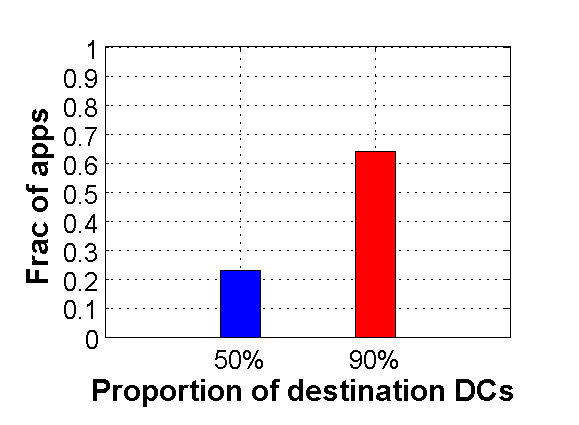
\includegraphics[width=\textwidth]{images/destinationDC.eps}%NeedMulticast.m
                \caption{\% of multicast transfers destined to \% of DCs.}
                \label{fig:bulk:dest}
        \end{subfigure}
	\hspace{0.1cm}
        \begin{subfigure}[b]{0.23\textwidth}
                \centering
                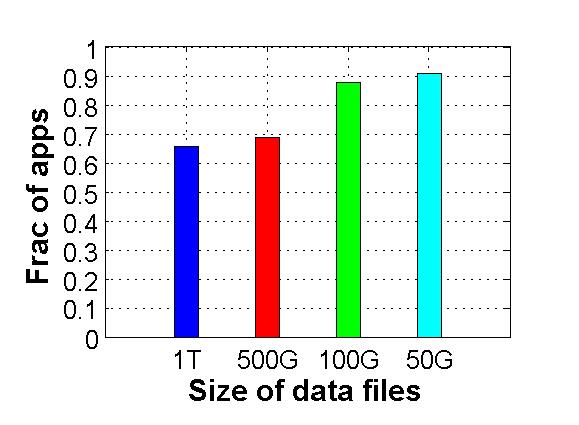
\includegraphics[width=\textwidth]{images/DataSize.eps}
                \caption{\% of multicast transfers larger than certain threshold.}
                \label{fig:bulk:size}
        \end{subfigure}
        \caption{Inter-DC multicast data transfers are (1) destined to a significant
fraction of DCs, and (2) huge in volume.}
        \label{fig:bulk}
\vspace{-0.4cm}
\end{figure}

\mypara{Destined to many DCs}
%<<<<<<< HEAD
Next, we examine whether these transfers are destined to
a large fraction (or just a handful) of DCs.
Figure~\ref{fig:bulk:dest} sketches the distribution of the
percentage of DCs (in total, $\sim$ 30) to which multicast
transfers in \company are destined.
%=======
%In the premise that multicast traffic amount to a substantial
%fraction of traffic, we then examine whether these transfers
%are destined to just a handful of DCs.
%Figure~\ref{fig:bulk:dest} sketches the distribution of the
%percentage of DCs (in total, $\sim$ 30) to which multicast
%transfers are destined.
%>>>>>>> 09029e454f71e5a5e01f13f554477705e665f4ec
We can see that about 90\% of multicast transfers replicate data
to more than 60\% of DCs, and about 70\% of them are destined
to more than 80\% of DCs.
%<<<<<<< HEAD
Moreover, we also observed a great diversity  in terms of
source DCs and the sets of destination DCs (not shown here).
Together, these observations suggest that {\em it is untenable
to preconfigure the data transfer for each possible multicast
request.}
%=======
%Moreover, we observed a great diversity (not shown)
%in terms of source DCs and the sets of destination DCs.
%Together, these observations suggest that it is undesirable to
%pre-configure the multicast overlay.
%>>>>>>> 09029e454f71e5a5e01f13f554477705e665f4ec

%In the premise that bulk data shares a large fraction of overall traffic, we check the number of destination DCs of the data. Fig. \ref{fig:bulk:dest} shows that there are over 60\% applications with bulk data multicast traffic are destined to at least 90\% DCs, and about 20\% applications with bulk data destined to over 50\% (but less than 90\%) DCs. These results show that a large fraction of the bulk data traffic is multicast to almost all DCs.

\mypara{Carrying bulk data}
Finally, we examine the data sizes of inter-DC
multicast transfers.
Figure~\ref{fig:bulk:size} sketches the distribution of the
size of data files that need to be multicast in \company.
We see that over 60\% of multicast data files are larger than 1TB,
while 90\% of them are larger than 50GB.
%<<<<<<< HEAD
Such large data volumes suggest that the transfers are usually
long-lived, and thus {\em we should dynamically adjust
the routing scheme during a data transfer in response to
dynamic network performance.}
%=======
%The large data volumes suggest that the transfers are usually
%long-lived and thus we could improve multicast performance by
%routing data adaptively during a data transfer in response to
%dynamic network performance.
%>>>>>>> 09029e454f71e5a5e01f13f554477705e665f4ec


\vspace{0.1cm}
These findings indicate a strong need for a systematic approach
to optimizing inter-DC bulk-data multicast.

%To further explore the characteristics of the multicast data files, we summarize the data size of these files and present the statistical results in Fig. \ref{fig:bulk:size}, which shows that nearly 70\% applications have a data file larger than 1TB and over 90\% of these multicast applications have data files larger than 50GB. Thus, focusing on optimizing bulk data multicast transmission is quite valuable to improve WAN conditions.

%\begin{itemize}
%
%\item Share of multicast traffic: use a bar chart to show the breakdown of all Baidu's total traffic volume into non-multicast traffic, and the multicast traffic of each application. {\em This should show a large fraction of traffic is multicast, and they are from many different applications.}
%
%\item A CDF of number of destination DCs. {\em This should show that most multicast traffic are destined to almost all DCs.}
%
%\item A CDF of size of multicast data files. {\em This should show that most multicast data are bulk data (not small data), and thus focusing on optimizing bulk data multicast is valuable.}
%
%\end{itemize}

\subsection{A case for inter-DC multicast overlay}
\label{subsec:motivation:case-for}

%\begin{figure}[t]
%\centering
%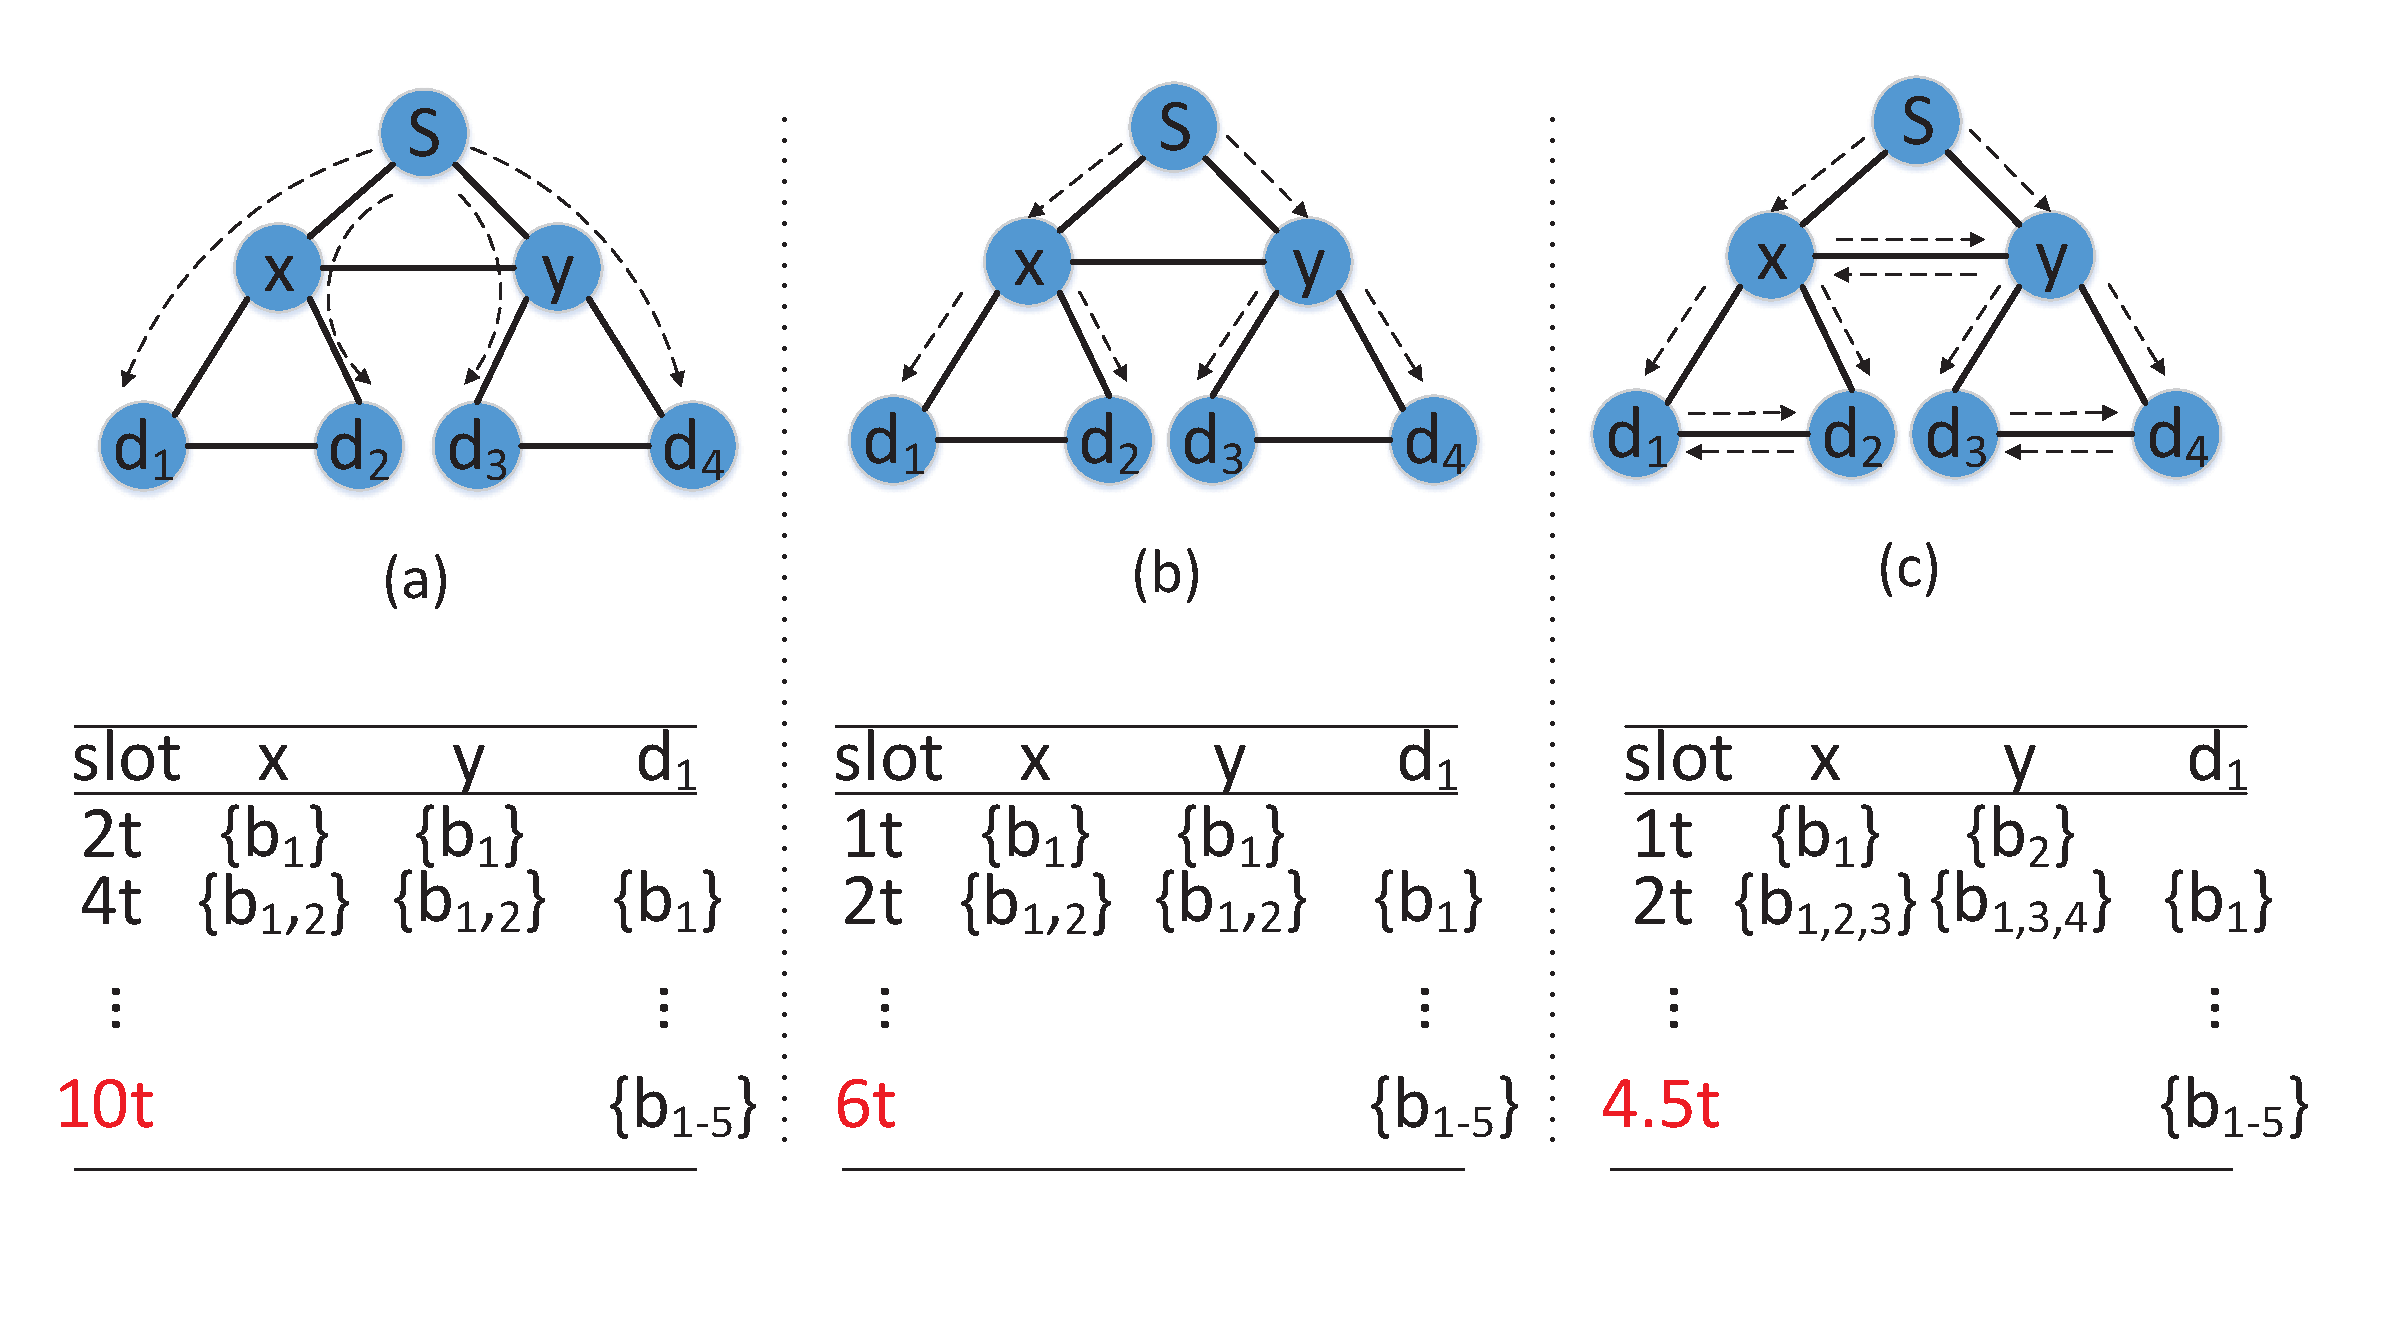
\includegraphics[width=80mm]{images/example.eps}
%\caption{A toy example showing the benefit from inter-DC multicast overlay.}
%\label{fig:case:example}
%\vspace{-0.4cm}
%\end{figure}

\begin{figure}[t]
\centering
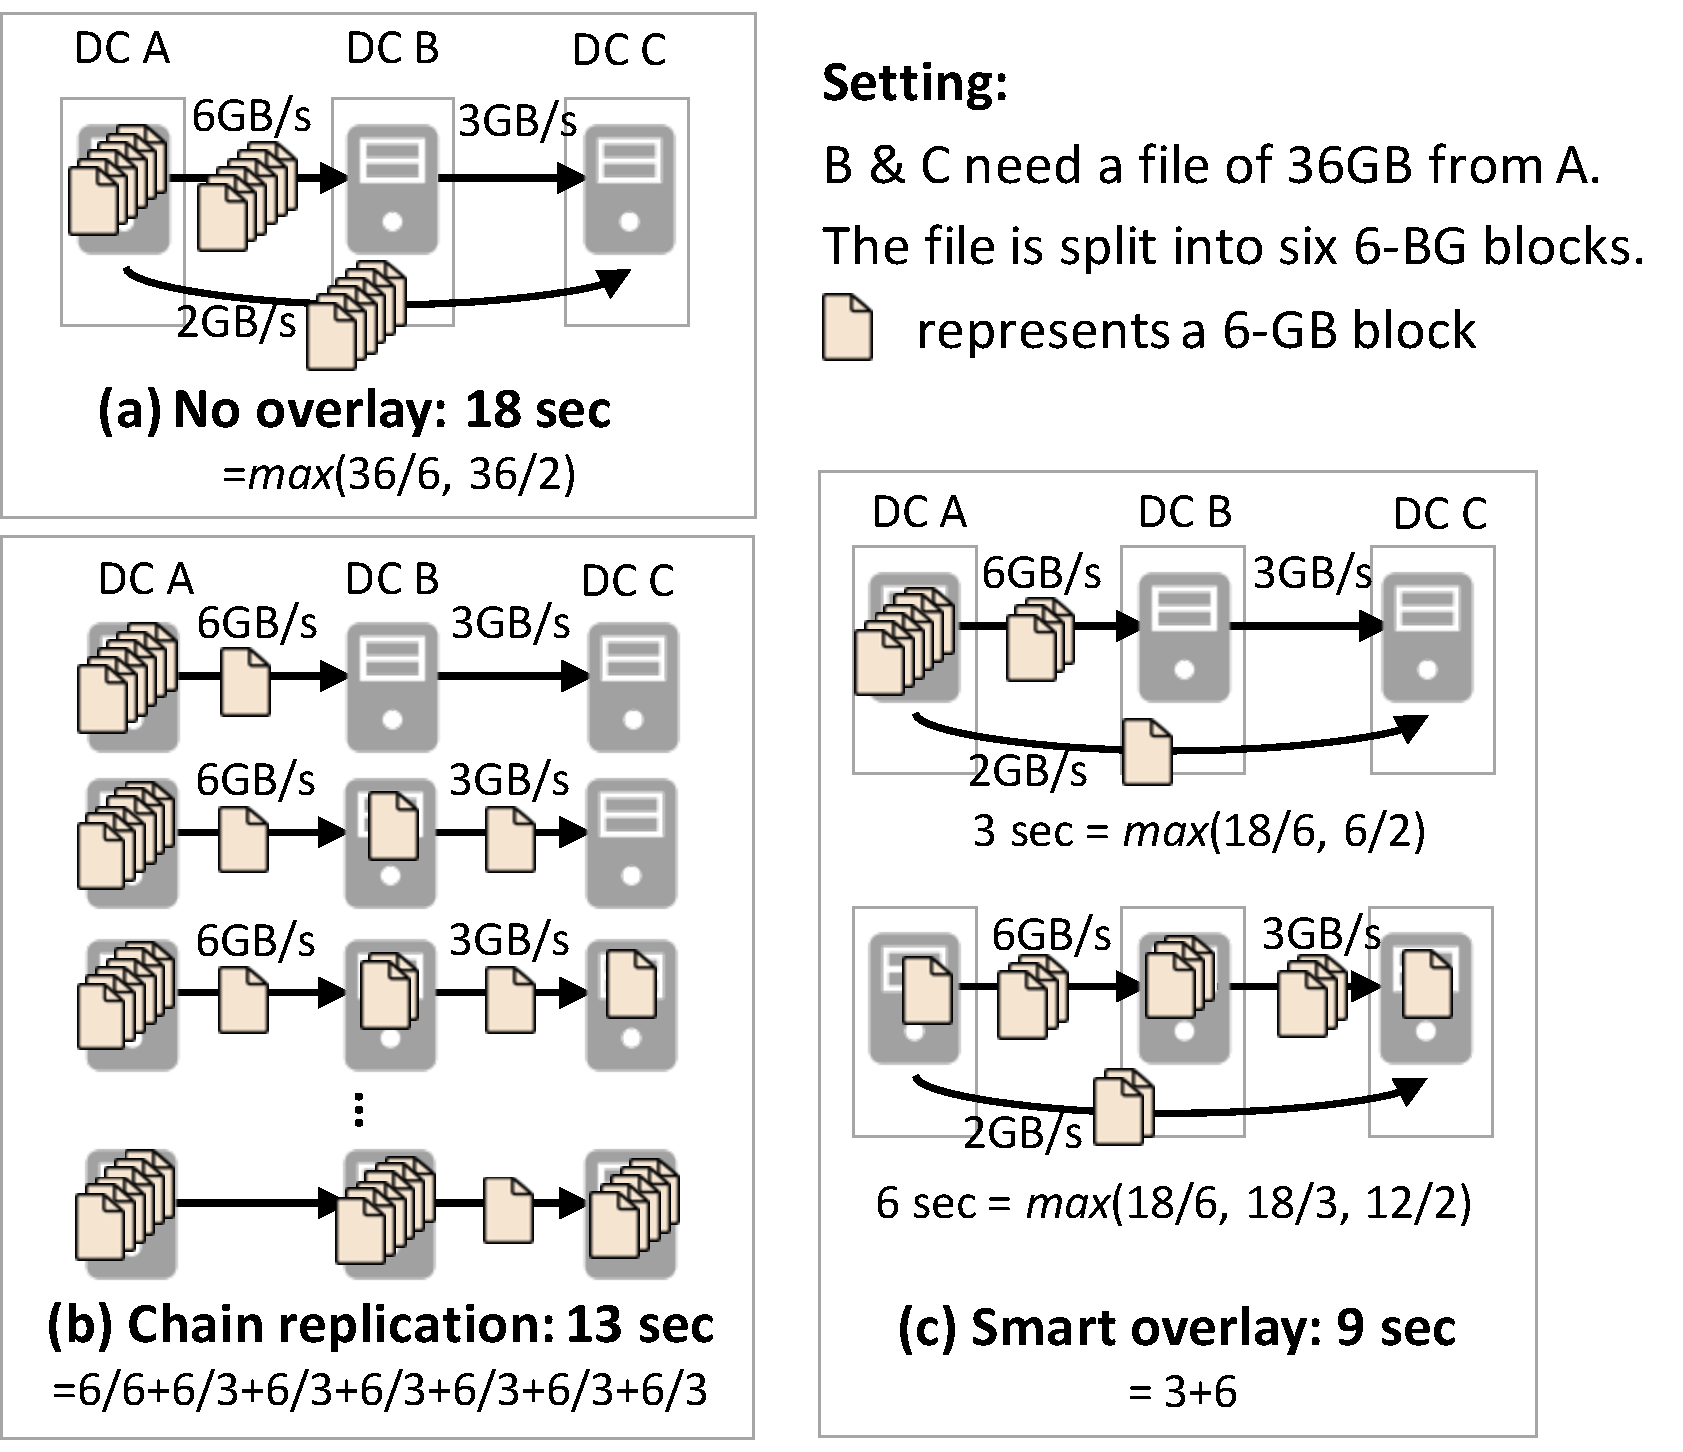
\includegraphics[width=80mm]{images/example-junchen.pdf}
\caption{A toy example showing the benefit from inter-DC multicast overlay.}
\label{fig:case:example}
\vspace{-0.4cm}
\end{figure}

In general, it is well-known that multicast over WANs can benefit
from an application-level overlays.
Here, we demonstrate, first by an illustrative example and then by
real-world measurement, that similar ideas could lead to
substantial improvement in inter-DC bulk-data multicast.

\mypara{An illustrative example}
As shown in Figure~\ref{fig:case:example},
suppose DC $B$ and $C$ want to fetch from DC $A$ a 36GB data file,
which is split into six 6GB blocks.
(The transfer is completed as long as the data is fully received
by some servers in $B$ and $C$.)
%<<<<<<< HEAD
Topologically, $A$ is directly connected with $B$ by a 2GB/s
link, and $A$ has two paths to reach $C$: the WAN path
which has 2GB/s capacity
(note that this path could go through $B$), or an overlay path
from $A$ first to a server $b$ in $B$ with a 6BG/s link,
and then from $b$ to $C$ with a 3GB/s link.
To begin with, if $A$ sends the data directly to $B$ and $C$,
i.e., no application-level overlay,
as in Figure~\ref{fig:case:example}(b),
the completion time would be 18 seconds.
If we apply the idea of application-level overlay but with
a simple DC-level chain
%=======
%Topologically, $A$ is directly connected to $B$, and
%$A$ has two paths to reach $C$: the WAN path
%which has 2GB/s capacity
%(note that this path could go through $B$), or the overlay path
%from $A$ to a server $X$ in $B$ with 6BG/s capacity,
%and then from $X$ to $C$ with 3GB/s capacity.
%To begin with, if $A$ sends the data directly to $B$ and $C$,
%as in Figure~\ref{fig:case:example}(a),
%i.e., no application-level overlay,
%the the completion time would be 18 seconds.
%If we use overlay routing but only with a simple DC-level chain
%>>>>>>> 09029e454f71e5a5e01f13f554477705e665f4ec
replication scheme, as shown in Figure~\ref{fig:case:example}(c),
it would take 13 seconds
to complete, already a 27\% decrease from 18 seconds.
However, we can further reduce the completion time
by judiciously scheduling blocks on different
overlay paths. For instance, Figure~\ref{fig:case:example}(d)
illustrates an overlay routing scheme which completes in 9
seconds, another 30\% decrease from 13 seconds.

The example of Figure~\ref{fig:case:example}
reveals a key (and well-known) observation that
{\em the benefits of
application-level overlay networks depend critically on if
there exist disjoint paths between two nodes.}


%Fig. \ref{fig:case:example} shows three cases under different transmission strategies. Assume there are 6 DCs in the network: source DC \emph{S}, 2 intermediate DCs \emph{X} and \emph{Y}, 4 destination DCs $d_1,d_2,d_3,d_4$, and the bandwidth of both upload and download links are all 2Gbps. There is a 5G data file in the source DC \emph{S} that should be multicasted to all the 4 destination DCs. The data file is split into 5 blocks ($b_1,b_2,b_3,b_4,b_5$) each with 1G-size. (a) Directly sending data to each destination DC. The four source and destination pairs (s,d) share the link bandwidth fairly, and each is allocated to 0.5Gbps. Thus, the overall completion time in $d_i$ is 10t. (b) Build a multicast tree with chain replications on the intermediate DCs. Take $d_1$ as an example, his parent DC \emph{X} could begins to send $b_1$ with 1Gbps at the beginning of 2nd time slot because \emph{X} has already duplicated $b_1$ after 1t. So that the completion time can be reduced to 6t. (c) An optimal solution on multicast overlay network. \emph{S} sends different blocks to \emph{X} and \emph{Y} in the 1st time slot to make them share those block mutually in the next slot. Thus, in the end of 2nd slot, both \emph{X} and \emph{Y} have 3 blocks. Similarly, $d_1$ and $d_2$ are also able to share complementary blocks while download the other blocks from parent DC simultaneously. The completion time can then be further reduced to 4.5t.

\begin{figure}[t]
\centering
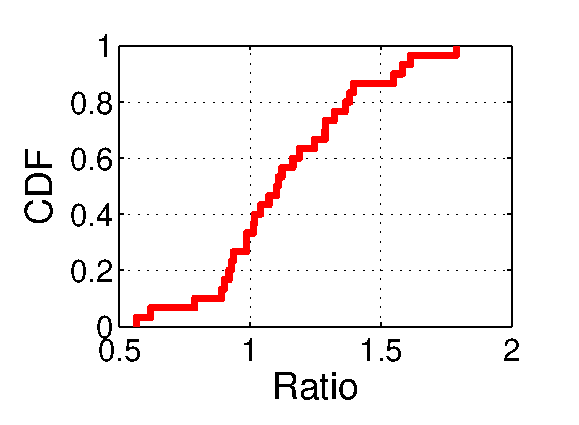
\includegraphics[width=1.5in]{images/potential_v2.eps}%DrawUp.m
\caption{The ratio between the available bandwidth
from $A$ to $C$ through WAN ($BW_{A\rightarrow C}$) and
that from $A$ to $C$ through $b$
($BW_{A\rightarrow b\rightarrow C}$),
across all possible $b$.}
%\jc{drop (a). avoid using notions in figure captions. captions should be standalone}\jc{please use notations in consistent with those in the text}
\label{fig:case:size}
\vspace{-0.4cm}
\end{figure}

%<<<<<<< HEAD
\mypara{Inter-DC path diversity}
We argue that the benefits illustrated in the example of
Figure~\ref{fig:case:example} can be actually realized in a
real DC WAN. The intuition is that
global-scale online service providers,
such as Google and \company, have disjoint paths in abundance,
both at DC-level (e.g., consider B4~\cite{jain2013b4}'s WAN topology)
and at server-level (e.g., consider Figure~\ref{fig:case:example}
where depending on the intermediate server $b$ in $B$,
$A$ has many overlay paths to $C$).

A crucial question, however, is that while two overlay paths are
physically disjoint, they might share the same bottleneck, and
thus should be counted as not disjoint in our context.
While sharing bottleneck is unlikely when two paths go through
different sequence of DCs,
when two overlay paths go through different servers but traverse
the inter-DC WAN path, they would tend to have the same network
bottlenecks, as WAN capacity is usually believed to be more
limited than intra-DC networks.
However, as shown in Figure \ref{fig:case:size}, our empirical measurement in \company's networks shows
otherwise.
We consider three DCs from \company's WAN that have the same
connectivity as in Figure~\ref{fig:case:example},
and show the distribution of
$\frac{BW_{A\rightarrow C}}{BW_{A\rightarrow b\rightarrow C}}$,
the ratio between the available bandwidth
from $A$ to $C$ through WAN ($BW_{A\rightarrow C}$) and
that from $A$ to $C$ through $b$
($BW_{A\rightarrow b\rightarrow C}$),
across all possible choices of $b$.
If WAN is indeed the bandwidth bottleneck, we should see
$\frac{BW_{A\rightarrow C}}{BW_{A\rightarrow b\rightarrow C}}=1$,
but the graph shows a substantial discrepancy between
$BW_{A\rightarrow C}$ and $BW_{A\rightarrow b\rightarrow C}$,
indicating that the available bandwidth can be bottlenecked by
the capacity of server $b$
($BW_{A\rightarrow C}>BW_{A\rightarrow b\rightarrow C}$),
or the intra-DC network in DC $B$
($BW_{A\rightarrow C}<BW_{A\rightarrow b\rightarrow C}$).
These observations corroborate the intuition that
{\em many physically
disjoint overlay paths tend not to share bottleneck}.

%=======
%\mypara{Opportunities in the wild}
%Next, we use performance measured from \company's DC servers to
%investigate whether the benefits illustrated by
%Figure~\ref{fig:case:example} can be realized in a real DC WAN.
%The example of Figure~\ref{fig:case:example}
%reveals a well-known observation that the benefits of
%application-level overlay networks depend critically on if
%there exist disjoint paths between two nodes that have diverse
%performance.
%We argue that global-scale online service providers such as Google
%and \company have such disjoint paths in abundance.
%First, the disjoint paths can emerge both
%at DC-level (e.g., consider B4~\cite{b4}'s WAN topology) and
%at server-level (e.g., consider Figure~\ref{fig:case:example}
%where depending on the intermediate server in $B$,
%$A$ has many overlay paths to $C$, all via the same DC-level
%path).
%Next, we use Figure~\ref{fig:case:size} show that these paths
%have substantially diverse performance.
%We consider three DCs from \company's WAN that have the same
%connectivity as in Figure~\ref{fig:case:example}.
%We randomly selected
%>>>>>>> 09029e454f71e5a5e01f13f554477705e665f4ec


%Consider the abstract topology of \company's real network, we can also find the situations similar to the above example. There are several DC groups divided by geographical locations, and every two groups are connected through one fiber link with high bandwidth. Within each DC group, there are dozens of DCs, and in each DC, there are normally 10,000 servers. Thus, there are numbers of possible disjoint paths between any DC pairs.

%To intuitively show the benefit from disjoint paths, we make the follow measurements on the available bandwidth among three DC groups \emph{X, Y, B}. The topology is shown in Fig. \ref{fig:case:size}(a). $x_i,y_i$ and $b_i$ are servers in \emph{X, Y, B}, while any server in \emph{X} needs to go through \emph{Y} to get to any arbitrary server $b$ in \emph{B}. Let $bw(XYB)$, $bw(YB)$ denote the bandwidth between $x_i$ and $b_k$, and between $y_j$ and $b_k$, respectively, we show the fraction of $bw(XYB)$ and $bw(YB)$ in Fig. \ref{fig:case:size}(b). This figure illustrates that only in a few case (about 20\%), the available bandwidth between \emph{Y} and \emph{B} is higher than that between \emph{X} and \emph{B}, while in the majority of cases, $\frac{bw(XYB)}{bw(YB)}>1$, meaning selecting senders is not straightforward, and we do need to consider large decision spaces.

%\begin{itemize}
%
%\item Give an illustrative toy example to compare (1) directly sending data to each destination DC, (2) use chain replication, i.e., build a multicast tree with each DC being a node, (3) an optimal solution.
%{\em\bf This example is critical!}
%
%\item Briefly explain the basics of Baidu's inter-DC WAN: topology, \# of servers per DC, some estimates on how many disjoint paths are available between two DCs.
%{\em The point is that each DC has multiple disjoint paths to fetch data, despite a seemingly tree-like topology.}
%
%\item Show a CDF of $\frac{X_i\rightarrow B}{Y_i\rightarrow B}$, where $X_i\rightarrow B$, $Y_j\rightarrow B$ are the bandwidth between some server in $X$ and $B$, and between some server in $Y$ and $B$, respectively. Assume $X$ needs to go through $Y$ to get to $B$.
%{\em The point is that in a substantial fraction of cases, $\frac{X_i\rightarrow B}{Y_i\rightarrow B}>1$, meaning selecting the sender is not straightforward, we do need to consider large decision space.}
%
%\end{itemize}

\subsection{Limitations of existing solutions}
\label{subsec:motivation:baseline}


We have seen that inter-DC multicast overlay networks have
promising potentials in optimizing inter-DC bulk-data multicast.
Realizing such potential in practice, however,
is easier said than done.
At a first glance, it seems we can borrow existing techniques
from other multicast overlay systems, which logically solves a
similar problem.
However, drawing on \company's experience deploying and evolving
its multicast overlay networks, we identify two limitations of
applying existing multicast overlay protocols in inter-DC bulk
data multicast.

\mypara{Existing solutions}
A few years ago, to meet the need of rapid growth in multicast
data, \company deployed a simple
receiver-driven decentralized protocol, which
was similar to what was used in other overlay networks
(such as CDNs and overlay video streaming)
where multicast is needed.
Since then \company has refined and improved the performance of
this solution, but the basic workflow of
data requests remains the same.
When multiple DC wants to download a data
file, they send the request to the source DC, and then the
requested data would flow back through multiple stages of
intermediate servers, where the selection of senders in each stage
is driven by the receivers of the next stage in a decentralized
fashion.
This basic workflow resembles many state-of-the-arts overlay
protocols designed for large-scale live video
streaming~\cite{Andreev2013Designing,sripanidkulchai2004analysis,zhang2005coolstreaming}.
%For the intermediate DCs, there is a customized store-and-forward strategy that decides whether to store the data or not and when to delete the data.
%The being used protocol in \company is a receiver-driven decentralized protocol. Once a receiver wants to download a data file, it announces the requirement to the source DC, then the required data will be forwarded to it through both the source DC and intermediate DCs. For the intermediate DCs, there is a customized store-and-forward strategy that decides whether to store the data or not and when to delete the data.
%This solution has been running for more than five years and has been continuously improved over time.

%At the same time, there are also some other solutions. For example, layered structures of DCs \cite{??} could simplify the scheduling and routing algorithm in the latency-sensitive systems but cannot explore more potential spaces and thus far from being optimal. Some pair-wise solutions like \cite{b4,bwe} improving inter-DC scheduling and routing are also not sufficient in the multicast overlay networks, due to the ignorance of multiple overlay paths.

%\mypara{Key limitations}
%To sum up, we can get two key lessons from the current baseline solutions.
As the inter-DC traffic continues to explode and more DCs are
deployed, this protocol has begun to show two limitations.


%\begin{figure}[t]
%        \centering
%        \begin{subfigure}[b]{0.23\textwidth}
%                \centering
%                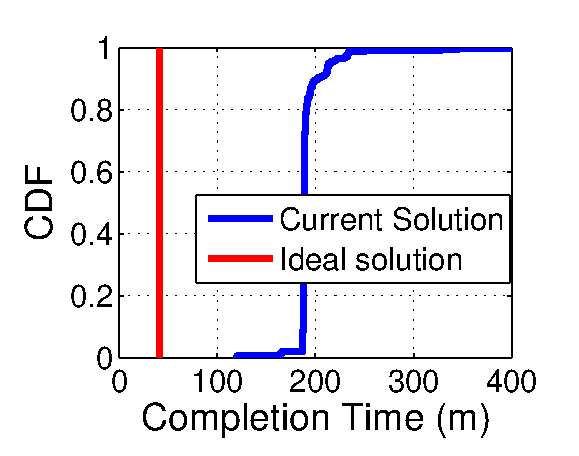
\includegraphics[width=\textwidth]{images/SEvsIdeal.eps}
%                \caption{The completion time of the 643 servers.}
%                \label{fig:motivation:observation1}
%        \end{subfigure}
%        \begin{subfigure}[b]{0.23\textwidth}
%                \centering
%                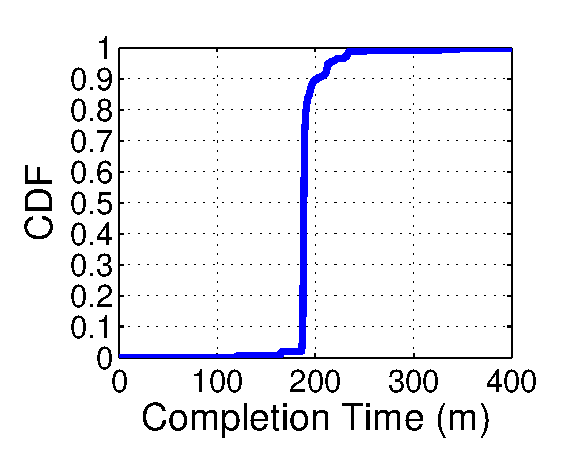
\includegraphics[width=\textwidth]{images/SE_3_cdf.eps}
%                \caption{The CDF of transmission completion time.}
%                \label{fig:motivation:observation2}
%        \end{subfigure}
%        \caption{The completion time under the current baseline solution. \jc{drop (b). add a line of 41minutes to (a). }}
%        \label{fig:motivation}
%\vspace{-0.4cm}
%\end{figure}

%\begin{itemize}
%\item Briefly describe how \company does multicast today: how to data is forwarded through an intermediate DC? what's the protocol (a receiver-driven decentralized protocol)?
%We should also stress that this solution has been running for \fillme years and has been continuously improved over time.
%
%\item Briefly mention other solutions (layered structure, hybrid approach, and why not optimizing pair-wise DC link is not sufficient)

%\jc{overall, these limitations need a bit elevation, and need to tie
%to the existing decentralized design}

\noindent{\bf Limitation 1:
Inefficiency due to the price of anarchy.}
The existing decentralized protocol lacks the global information
about the whole network, and thus cannot make optimal scheduling.
To show this, we run an experiment under a simplest topology in \name's network using real traffic trace.
There is 1 source DC and 2 destination DCs 
(there are 640 servers in each DC), and the data need to be transferred is 30GB, with 20Mbps upload and download
bandwidth on each server.
Theoretically, the optimal overlay solution could always select
the better source for any block of the data file, and the ideal
completion time for destination DCs is
$\frac{30\times 1024}{640\times 20Mbps \times 60s/min} = 41$
minutes.
Figure~\ref{fig:motivation} shows the results under the existing
protocol. We see that the average completion time is about
195 minutes, 4.75$\times$ longer than the optimal completion time.
What's worse, it also exhibits heavy tail latency and there are
about 5\% servers whose completion time is more than $200min$. Such inefficiency is due to the unreasonable selection of data source (probably with limited bandwidth or poor connections). Without a global view, the existing decentralized protocol in anarchy cannot explore the whole decision space to find the most efficient data source.


\begin{figure}[t]
  \centering
  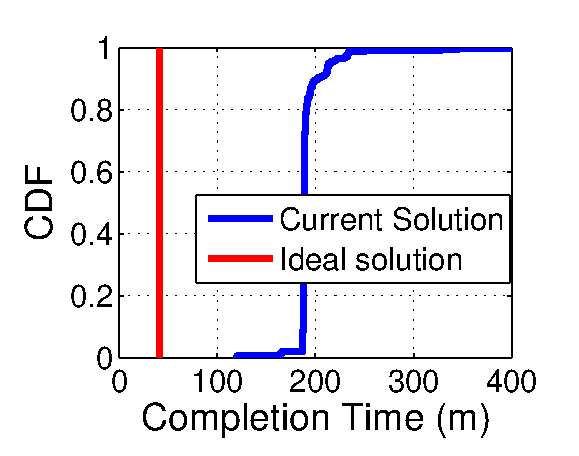
\includegraphics[width=45mm]{images/SEvsIdeal.eps}
  \caption{The real and ideal completion time of servers in destination DC.}
  \label{fig:motivation}
\vspace{-0.4cm}
\end{figure}

%\jc{this is still a toy example. we want to use real data to show these observations. how about using the previous figure to show tail latency.}

\noindent{\bf Limitation 2:
Interference with latency-sensitive traffic.}
The existing multicast overlay network share the same inter-DC WAN
with latency-sensitive traffic.
Despite using standard QoS technique and giving the lowest priority to
bulk data transfers, we still see frequent interference with
latency-sensitive traffic caused by bursty arrival of bulk data
requests.
We continuously monitored the bandwidth utilization of an inter-DC
link in four days where there is a bulk data transfer at 11:00 on the
2nd day (lasted for 6 hours and finished at 17:00).
Figure~\ref{fig:lesson2} shows the link utilization during the two
days, from which we can see that the bulk data transfer caused
obviously irregular traffic. As a result, the latency-sensitive online
traffic that runs simultaneously on this link therefore suffered over
30 times longer delay, usually speaking,
from about $15ms$ to nearly $500ms$. The reason of such inefficiency is that in a decentralized manner, although all the servers worked under the standard QoS requirements, the exceeding bandwidth usage of the inter-DC link still cannot be prevented due to the invisibility of global traffic.


\begin{figure}[t]
        \center
        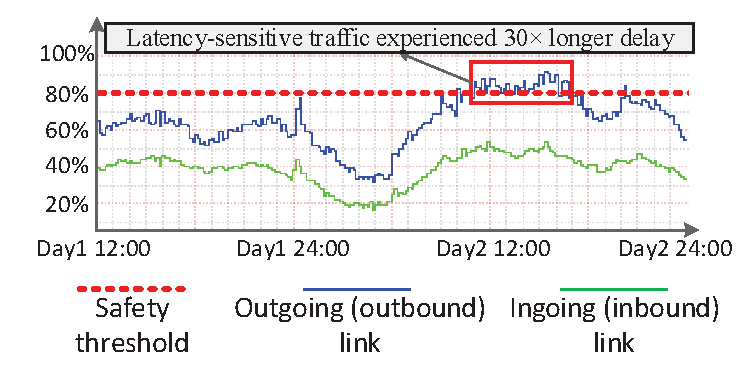
\includegraphics[width=3in]{images/nj02-M2A_0212-0216_v2.eps}
        \caption{Bulk data transfer on the 2nd day caused obviously irregular traffic.\jc{what's green line and blue line?? unclear from the figure why the boxed period has bad performance of latency-sensitive traffic. please add a horizontal line at 80\%, and an arrow with the text like ``Latency-sensitive traffic experienced 30$\times$ longer delay''}}
        \label{fig:lesson2}
%\vspace{0.1in}
\end{figure}

%\jc{can you say something like: such inefficiency is due to the inability
%to prevent exceeding bandwidth usage by bulk-data transfers in a
%decentralized manner}
%(1) Use a figure to show that bulk data transfer can cause significant delay on latency-sensitive traffic, and (2) put some concrete numbers to show such delay can cause significant revenue loss.

%\jc{can we show some numbers on how much delay on latency-sensitive traffic during that incident? and how much losses did it cause (either in terms of application quality or in \$\$)?}

%\end{itemize}

